\chapter{Cause specific mortality rates: alcohol dependence}
\label{applications-csmr}

A key assumption of the YLL estimates in GBD 2010 study is that only
one cause leads to death.  This categorical distribution of deaths
creates a rate that does not directly correspond to any rate in the
compartmental model (Figure \ref{forward-sim-two-compartment}) by
assuming those who die \emph{with} the condition die \emph{of} the
condition.  While this is a reasonable assumption for many conditions
such as cirrhosis or diarrhea, it is not for conditions such as
Parkinson's disease or alcohol dependence.  TK this chapter compares
the results of assuming $f''=0$ and $f''\geq 0$.

Alcohol dependence is the dysfunctional pattern of alcohol consumption
that leads to physiological dependence and impaired control.  Like
cocaine dependence in Chapter \ref{applications-splines_knot_loc}, to
be diagnosed with alcohol dependence, three of more of the seven
substance dependence criteria defined by the American Psychiatric
Association on page \pageref{page:app-substance_dependence} must be
fulfilled within a twelve-month period. \cite{association_diagnostic_2000, hasin_prevalence_2007}
Systematic review yielded prevalence, excess mortality and
cause-specific mortality data as seen in Figure \ref{fig:app-alcohol
  data}.

    \begin{figure}[h]
        \begin{center}
            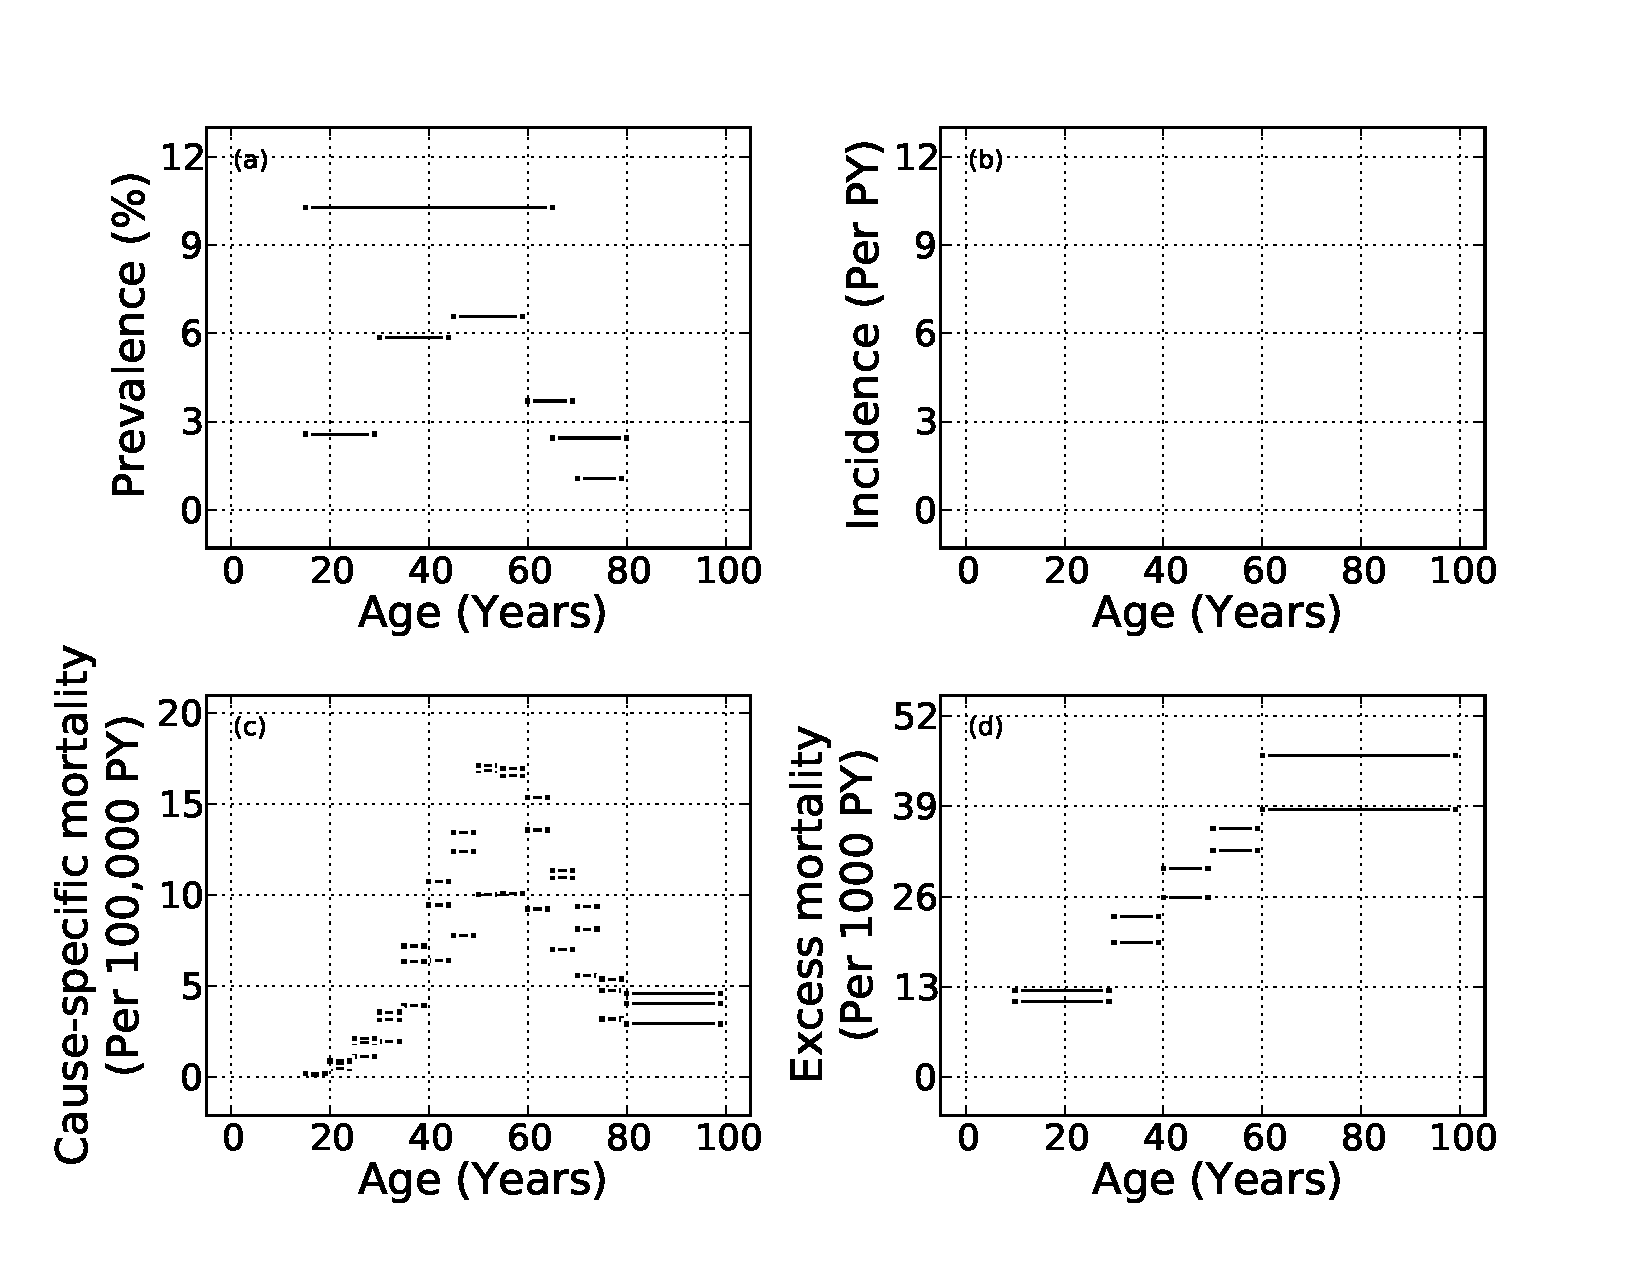
\includegraphics[width=\textwidth]{alcohol-data.pdf}
            \caption{Prevalence (panel (a)), incidence (panel (b)),
              cause-specific mortality (panel (c)) and excess
              mortality (panel (d)) of alcohol dependence in Western
              European males in 2005.}
            \label{fig:app-alcohol data}
        \end{center}
    \end{figure}

To include cause-specific mortality data in the compartmental model,
the model in Figure \ref{forward-sim-two-compartment} can be adapted
by splitting the excess mortality, $h_{f}$, into two parts (Figure
\ref{fig:two_compartment_2f})--those who die \emph{from} the
condition, $h_{f'}$, and those who die \emph{with} the condition but
\emph{not of} it, $h_{f''}$.  As described in Section
\ref{theory-csmr}, excess mortality can then be represented as the
following:
    \begin{equation}
        h_{f} = h_{f''} + h_{f'}
    \end{equation}
While the product of excess mortality and prevalence, $h_{p} \cdot h_{f}$,
can be directly measured, in practice $h_{f''}$ and $h_{f'}$ are never
disentangled.  This method implicitly separates $h_{f'}$ and $h_{f''}$
but does not try to explicitly represent both.

    \begin{figure}[h]
        \begin{center}
            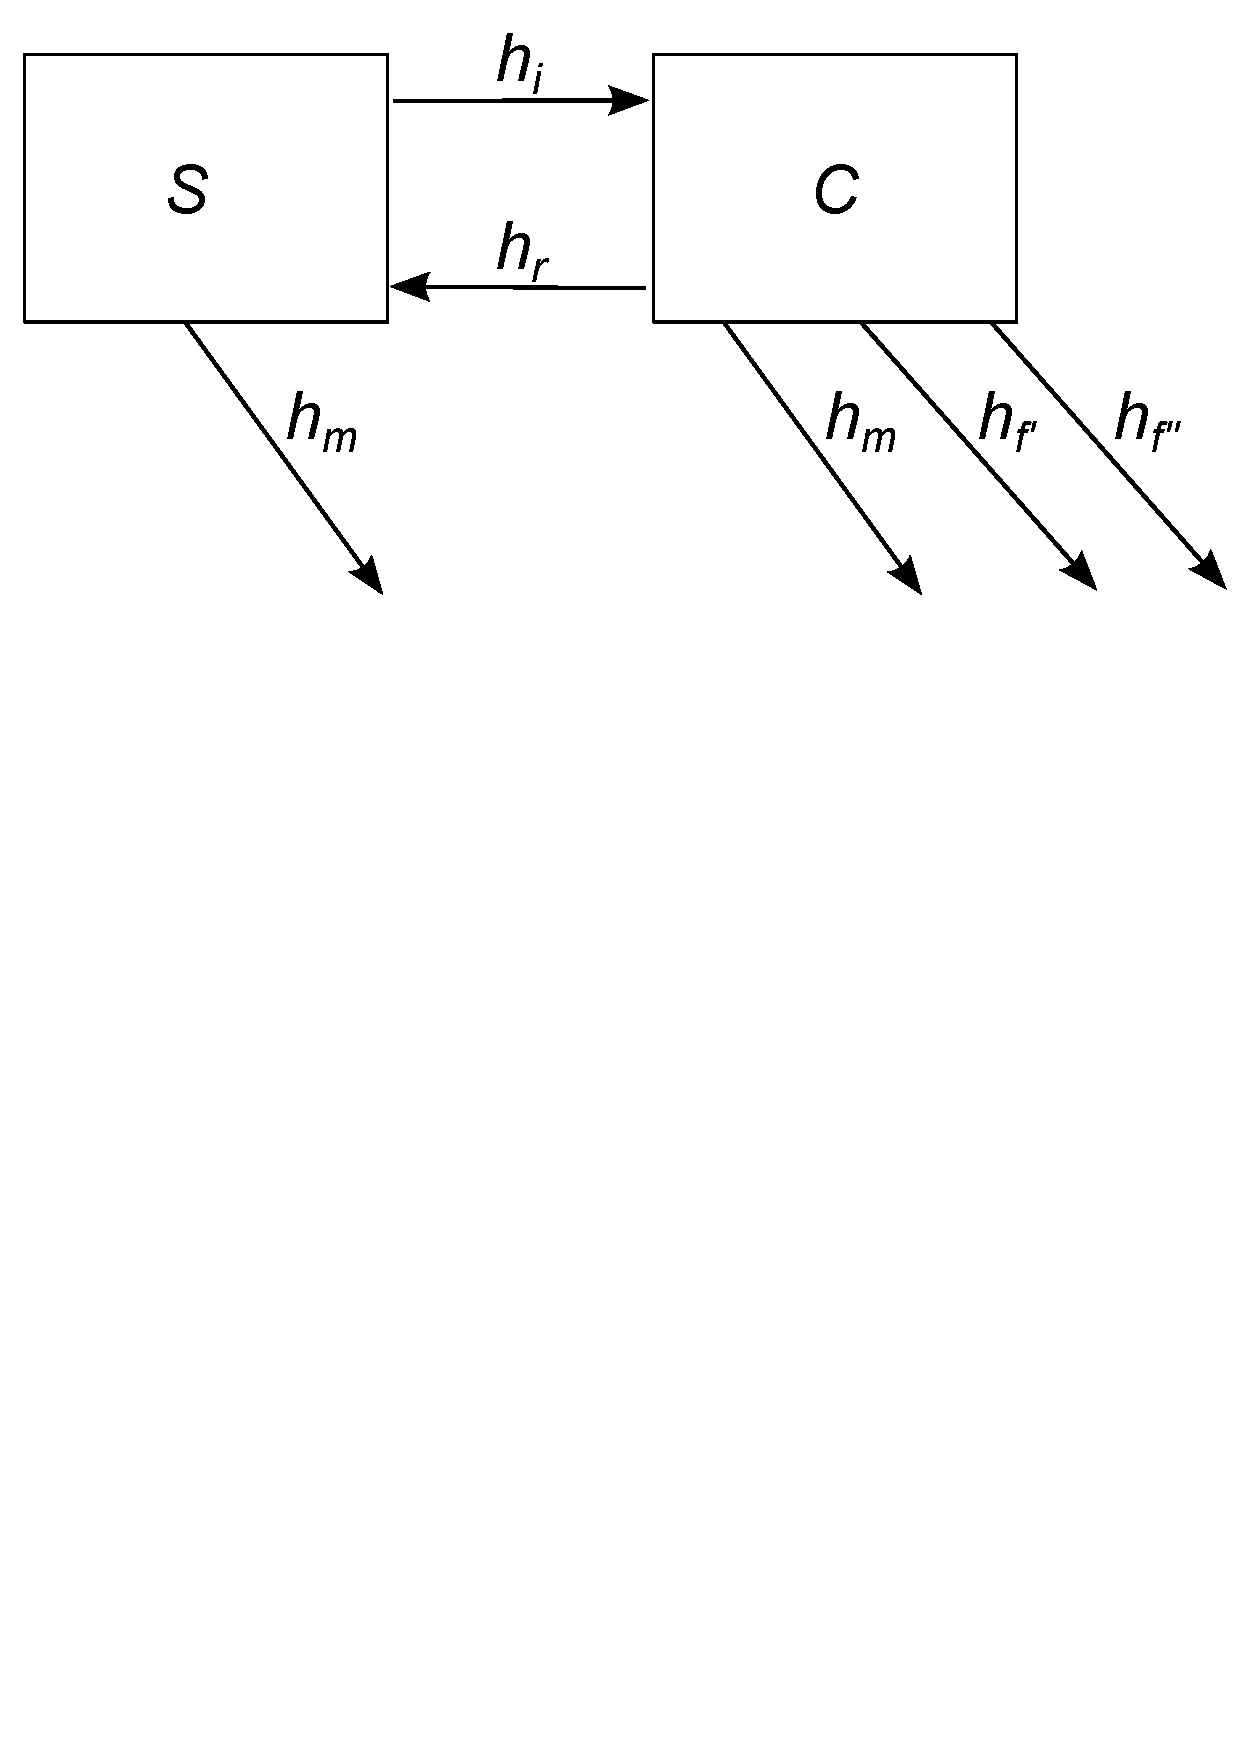
\includegraphics[width=\textwidth]{SC2.pdf}
            \caption{The two-compartment mechanistic model with the
              excess mortality split into two hazards.}
            \label{fig:two_compartment_2f}
        \end{center}
    \end{figure}

Many times in the GBD 2010 study, it is a reasonable assumption that
$h_{f''} = 0$, so that those who die with the condition die of it.
When this is the case, the cause-specific mortality is a direct
estimate of $h_{p} \cdot h_{f}$.  However, for diseases such as alcohol
dependence, this is a poor assumption, as many die with the condition
but not \emph{of} it.  When $h_{f''} \neq 0$, cause-specific mortality
data provide the lower bound of $h_{p} \cdot h_{f}$.  

As seen in Figure \ref{fig:app-alcohol compare}, modeling cause-specific mortality as
$h_{f''}$ (left column, panels (a), (c) and (e)) or as $h_{f'}$ (right
column, panels (b), (d) and (f)) only change the uncertainty of the
parameter estimates and elevates the cause-specific mortality
estimates while other parameter estimates remain the same.

    \begin{figure}[h]
        \begin{center}
            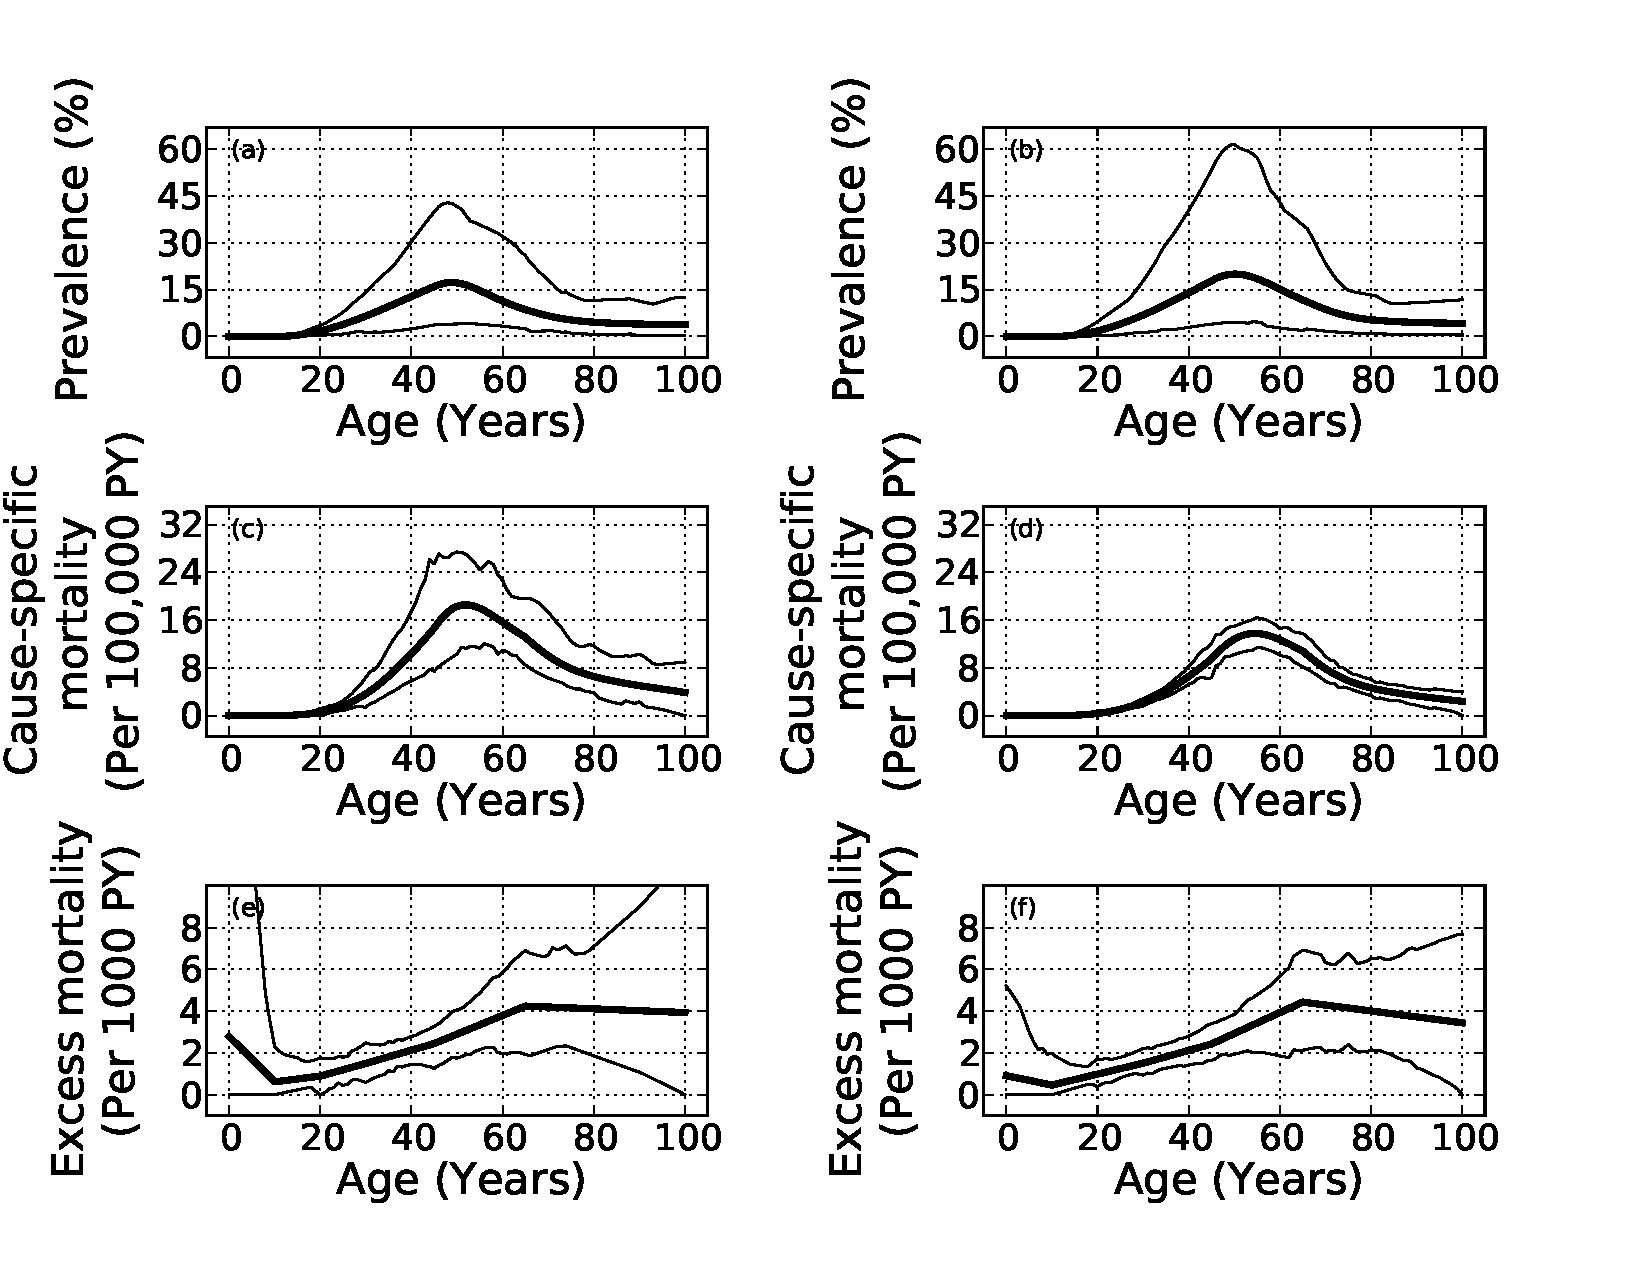
\includegraphics[width=\textwidth]{alcohol-csmr_v_pf.pdf}
            \caption{Comparison of prevalence (panels (a) and (b)),
              cause-specific mortality (panels (c) and (d)) and excess
              mortality (panels (e) and (f)) estimates of alcohol
              dependence in Western European males in 2005 when using
              cause-specific mortality data as a lower bound (panels
              (a, c, e)) or a direct estimate of the product of
              prevalence and excess mortality (panels (b, d, f)).}
            \label{fig:app-alcohol compare}
        \end{center}
    \end{figure}
    
This method allows the compartmental model in \ref{forward-sim-two-compartment}
to use the cause-specific mortality data that results from the ``one cause, one death''
GDB 2010 Study manta.
